%-----------------------------------------------------------------------------%
% Format and styling in this file originally created by 
% Carl E. Svensson 2010, updated by Adam J. Carmichael 2011,2012
%-----------------------------------------------------------------------------%
%
%- Document Makeup -----------------------------------------------------------%
%- (01) Notes from template author
%- (02) Document Class and Options
%- (03) Standard package includes and options
%- (04) Custom Definitions and Alterations
%- (05) Custom Commands
%- (06) Document title and other metadata
%- (07) Start Document Content
%- (07a) Misc Config
%
%
%- (01) Notes from carneeki@ -------------------------------------------------%
% NEATNESS:
%  Please keep the TeX neat. Best ways to do this:
%  (01) Don't indent
%  (02) Keep inside of 80 characters (it makes for nicer editing on small
%       laptops).
%  (03) Avoid whitespace between \section{} and other document elements. We
%       have %%%% comments for a reason!
%  (04) Use 2 (that's TWO) space characters to indent. NEVER use tab unless
%       your editor converts to to space chars.
%  (05) Maintain customisations in their respective sections.
%  (06) Comment everything. Bandwidth and diskspace are cheap these days, and
%       TeX compresses pretty nice. Anything else is the BAD kind of laziness
%       on your part.
%
% MULTILINE EQUATIONS:
%  Use \begin{align} instead of \begin{eqnarray}...
%  Details as to why are found at (tl;dr : it's just better...):
%  http://texblog.net/latex-archive/maths/eqnarray-align-environment/
% 
% BIBLIOGRAPHY: 
%  -> URLS: to generate the GUID for a reference that is for a URL, paste
%     the URL into goo.gl and then take only the suffix portion.
%
%  -> Wikipedia citations, simply copy + paste the citation from the
%     menu on the LHS.
%
%
% preamble.tex v 2012-05-29 2216AEDT
%- (02) Document Class and Options -------------------------------------------%
\documentclass[
%  pagesize,
  a4paper,
  pdftex,
%  fontsize=11pt,
%  draft=true,
  twoside,
]{report}
%
%\clip(-11.74,-31.43) rectangle (11.68,35.96);
%- (03) Standard package includes and options --------------------------------%
%\usepackage{draftwatermark} % draft watermark. Comment these 2 lines in final
%\SetWatermarkLightness{0.9} %
\usepackage{watermark}
\usepackage{amsthm}
\usepackage{amsmath}       % amsmath & amssymb are almost ALWAYS required.
\usepackage{amssymb}       %
\usepackage{gensymb}       % for the degrees circle!
\usepackage{txfonts}       % negated math symbols
%
%\usepackage{verbatim}     % multiline commenting ( c++ equiv /* ... */ )
%
\usepackage{color}
\usepackage{xcolor}         % pdflatex
\definecolor{neekiGrey}{RGB}{192,192,192}
\definecolor{neekiRed}{RGB}{172,40,41}
\definecolor{neekiBlue}{RGB}{62,70,157}
\definecolor{neekiGreen}{RGB}{39,171,39}
\definecolor{neekiPurple}{RGB}{105,39,171}
%
\usepackage{geometry}      % option for altering page dimensions if needed
%\usepackage[pdftex]{graphicx} % including image files for figures (ie
                              % non-[E]PS)
%                          % valid types: jpeg, png, pdf
\usepackage{wrapfig}       % the figures themselves
\usepackage[numbers,
square,
longnamesfirst
]{natbib}                  % prettybib
\usepackage[pdftex]{hyperref} % clickable TOC and refs
%\usepackage[all]{xy}      % category theory helpers
%\xyoption{all}            % category theory helpers
%\input xy                 % category theory helpers
\usepackage{pgf,tikz}      % easy graphic thing
\usepackage{tabularx}    % easy tables
\usepackage{url}         % easy urls
\usepackage{multirow}    %
\usepackage{lipsum}      % autogen placeholder text
\usepackage{datetime}    % insert current time (for title page)
%
%- (04) Custom Definitions and Alterations -----------------------------------%
\usepackage[T1]{fontenc} % font-doohickey
%\usepackage{tgadventor}  % font
%\usepackage[math]{iwona} % font
\usepackage{kurier} % font

\usetikzlibrary{arrows}

%
\linespread{1.5} % carneeki@ use approx 150% line spacing just like MaxDesign.
\hypersetup{
  % DO NOT CHANGE THESE
%   pdftitle={\metaTitle},
%   pdfauthor={\metaAuthorShort},
%   pdfsubject={\metaSubject},
%   pdfkeywords={\metaKeywords},
  pdfcreator={LaTeX},
  pdfproducer={LaTeX},
  pdftoolbar=false,
  % But change these to taste:
  pdffitwindow=false,   % window fit to page when opened
  pdfstartview={Fit},   % fits the width of the page to the window
                        % all (useful) opts: Fit, FitH, FitV,
  pdfpagelayout=TwoPageLeft,
  pdfnewwindow=true,    % open links in new window
  colorlinks=true,      % false = boxed links; true = colored links
  linkcolor=neekiRed, % color of internal links
  citecolor=neekiBlue, % color of links to bibliography
  filecolor=red, % color of file links
  urlcolor=red  % color of external links
}
\usepackage[Lenny]{fncychap}
%\usepackage[Bjornstrup]{fncychap}
%
%- (05) Custom Commands ------------------------------------------------------%
% MATH
%\newcommand{\derivative}[1][x]{\frac{\mathrm{d}}{\mathrm{d}#1}}
\newcommand{\nd}[1]{\,\mathrm{d}#1}
\newcommand{\md}[1]{\mathrm{d}#1}
\newcommand{\deriv}[2]{\frac{\nd{#1}}{\nd{#2}}} % derivative of fn
\newcommand{\lderiv}[2]{\deriv{}{#2}(#1)} % deriv of a long fn
\newcommand{\myint}[4]{\int_{#1}^{#2} #3~\d{#4}} % integrate
\newcommand{\aderiv}[2]{\myint{}{}{#1}{#2}}
\newcommand{\ndeg}{^\circ} % the degrees symbol
\newcommand{\neqref}[1]{\text{(#1)}}
% trig
\newcommand{\rsin}{\sin^{-1}}
\newcommand{\rcos}{\cos^{-1}}
\newcommand{\rtan}{\tan^{-1}}
\newcommand{\arcsec}{\operatorname{arcsec}}
\newcommand{\arccsc}{\operatorname{arccsc}}
\newcommand{\arccot}{\operatorname{arccot}}
% DMTH
\newcommand{\lxor}{\oplus}
\newcommand{\lxnor}{\lnot\lxor}
\newcommand{\true}{(\mathbb{T})}
\newcommand{\false}{(\mathbb{F})}
% GENERAL
\newcommand{\tsup}[1]{\textsuperscript{#1}}
\newcommand{\tsub}[1]{\textsubscript{#1}}
\newcommand{\qedbitches}{\qed}
\renewcommand{\labelenumi}{(\alph{enumi})}
\renewcommand{\labelenumii}{(\roman{enumii})}
%
%- (06) Document Title and other metadata ------------------------------------%
\thiswatermark{
% challenge accepted guy
% bottom right: (220,-760)
% bottom left: (-60,-760)
\put(-60,-760){
\begin{tikzpicture}
  \node[opacity=0.1]{
\includegraphics[scale=1.8]{img/challenge.jpg}};
\end{tikzpicture}
}
}
\title{
  KCMQ: Knack Central at Macquarie University \\
  Society Roadmap Meeting: 2012-06-21
}
%
\author{
  Carl E. Svensson \& \\
  Adam J. Carmichael \\
  Department of Engineering\\
  Macquarie University\\
  Sydney, Australia 2109\\
  Email: \url{carl.svensson@ieee.org} \\
  Email: \url{adam.carmichael@ieee.org}
}% author END Brace
%
%- (07) Start Document Content -----------------------------------------------%
\begin{document}
%- (07a) Misc Config ---------------------------------------------------------%
%
\maketitle
%
%\begin{abstract}
%This document is a guide written primarily by a MATH130 student and his friend
%in the 2 week study period between end of class and the examination of
%semester 1, 2011. It is an interpretation that aims to make the very thorough
%notes of Chen and Duong easier and more accessible to the rest of us.
%\end{abstract}
\tableofcontents
\chapter{}
\vspace*{\fill}
\begin{center}
This page is intentionally left blank.
\end{center}
\vspace*{\fill}
\section{Name and Acronym}
\label{sec:NameAndAcronym}
\subsection{Outcome}
\begin{description}
  \item[KCMQ:] Knack Central Macquarie University. The mission statement and
  many engineering themes revolve around \emph{knack}, and so we felt reflecting
  this in the name would be a good thing to tie in with the overall branding. It
  is also partly humourous, the Dilbert episode ``The Knack''.
\end{description}

Logo needs to be a simple vector of some description involving at most 4
colours, but multiple tones of colour are permissible. This is to keep printing
costs down, and to make the logo recogniseable.

Logo concepts include circuitry and tools to form letters for the acronym
``KCMQ'' with the motto being: ``Engineering Motto: Challenge Accepted''.

% \begin{figure}[!hbt]
% \label{fig:LogoIdea}
% \begin{tikzpicture}
%   \node[font=\big] at (1,1) {KCMQ};
% \end{tikzpicture}
% \caption{Logo Concept Idea}
% \end{figure}

\subsection{Other candidates}
\begin{description}
  \item[MESS:] Macquarie Engineering Student Society
  \item[MESS:] Macquarie Engineering and Science Society
  \item[MES:] Macquarie Engineering Society
  \item[SAME:] Students At Macquarie in Engineering
  \item[EMU:] Engineers/Engineering at Macquarie University
  \item[E=MQ$^2$:] Engineers/Engineering at Macquarie University
  \item[TEAM:] The Engineers At Macquarie University
  \item[MATE:] Macquarie And The Engineers
  \item[MEAL:]
  \item[LAME:]
  \item[MEAT:]
  \item[MEME:]
  \item[MEAD:]
\end{description}

\subsection{Action Items}
\begin{itemize}
  \item Seek objectors to name.
\end{itemize}
\section{Articles of Association}
\label{sec:ArticlesOfAssociation}
\subsection{Action Items}
\begin{itemize}
  \item Form articles of association document
  \item Modify charter (requires separate meeting)
  \item Get 15 students to sign up to join
  \item Determine initial committee and named office bearers
  \item Formalize branding
\end{itemize}
\section{Named positions And Role Descriptions}
\label{sec:NamedPositions}
\subsection{Outcome}
Structure will be a 3 tier system.
\begin{description}
  \item[Office Bearing Positions on Committee] Several named positions will bear
  an office and title.
  \begin{description}
    \item[Chief] - Executive office bearing position. Equivalent to a President
    of a society in function.
    \item[First Assistant Engineer] - Executive office bearing position.
    Equivalent to a secretary in function.
    \item[Second Assistant Engineer] - Executive office bearing position.
    Equivalent to a treasurer in function.
    \item[QMED - Marketing] - Office bearing position. QMED stands for
    ``Qualified Member of the Engine Department''.
    \item[QMED - Activities] - Office bearing position.
    \item[QMED - Partnerships] - Office bearing position.
    \item[QMED - PAL/Education] - Office bearing position.
    \item[QMED - Memberships] - Office bearing position.
    \item[QMED - IT \& Communications] - Office bearing position.
  \end{description}
  \item[Fitter] These are committee members with nonspecific functions. Required
  for committee meetings (voting), and to fill in for office bearing positions
  as needed.
  \item[General Members] (most people will fit into this category).
\end{description}

Executive committee members are the three members of the committee who are
responsible for the society to MUSRA. For example, they are the three nominated
signatories responsible for paperwork to MUSRA in the ``boot sequence'' for the society.

\subsection{Action Items}
\begin{itemize}
  \item Need to outline out the responsibilities of each role in greater detail.
\end{itemize}
\section{Committee \& Reporting Structures}
\label{sec:CommitteeAndReporting}
\subsection{Outcome}
\begin{itemize}
  \item Committee structure has been outlined in further detail in section
  \ref{sec:NamedPositions}, \nameref{sec:NamedPositions} on page
  \pageref{sec:NamedPositions}.
  \item Reporting
  \begin{itemize}
    \item Attendance at events \& activities
    \item Membership roster is handled well by Google Docs spreadsheet
    \item The executive to report to MUSRA, primary responsibility is to the
    Secretary, however, the Secretary may call upon assistance in reporting.
    \item Annual club report to be compiled by Chief and Treasurer to be
    distributed to club members via the website.
    \item Newsletter is a possibility, needs a dedicated committee member.
  \end{itemize}
\end{itemize}
\section{Mission Statement}
\label{sec:MissionStatement}
\subsection{Outcome}
Carl (predominantly) drafted a mission statement which reads as:\\

\emph{Furthing the enrichment and application of `knack' through a rich variety
of learning, social, and challenging activities for engineering (and like minded)
folk at Macquarie University.}\\
\\
%quote and quotation environments make following indentations look all munted
%todo: maybe fix that, if necessary.
\emph{`knack'} is to be linked to the famous\footnote{infamous?} Dilbert video
wherever possible where the Garbage Man defines \emph{'knack'} to be:\\

\emph{a rare condition characterized by an extreme intuition about all things
mechanical and electrical\ldots and utter social ineptitude.}

\subsection{Action items}
While we are largely happy with the mission statement as is, we are going to
allow ourselves more time to let creative juices mold it a little more (if they
are flowing).\\
\\
Also, peer review the mission statement before finalizing.

\section{Engineering Focusses}
\label{sec:focii}

\section{Outcome}
\begin{itemize}
  \item Amateur Radio
  \item MANETS - Mobile Ad-hoc Networks
  \item Robotics \& Mechatronics
  \item Embedded Computing
  \item Learning tools and techniques
  \item Applying Electronics
  \item PAL - Peer Assisted Learning
  \item Weekly Challenges
  \item Parent Student Body for Engineers
  \item Social activites
  \item Guest lecturers
  \item EWB Challenge
  \item Engineering Mentors
\end{itemize}

\section{Action Items}
\ldots
\section{Activities}
\label{sec:Activities}
%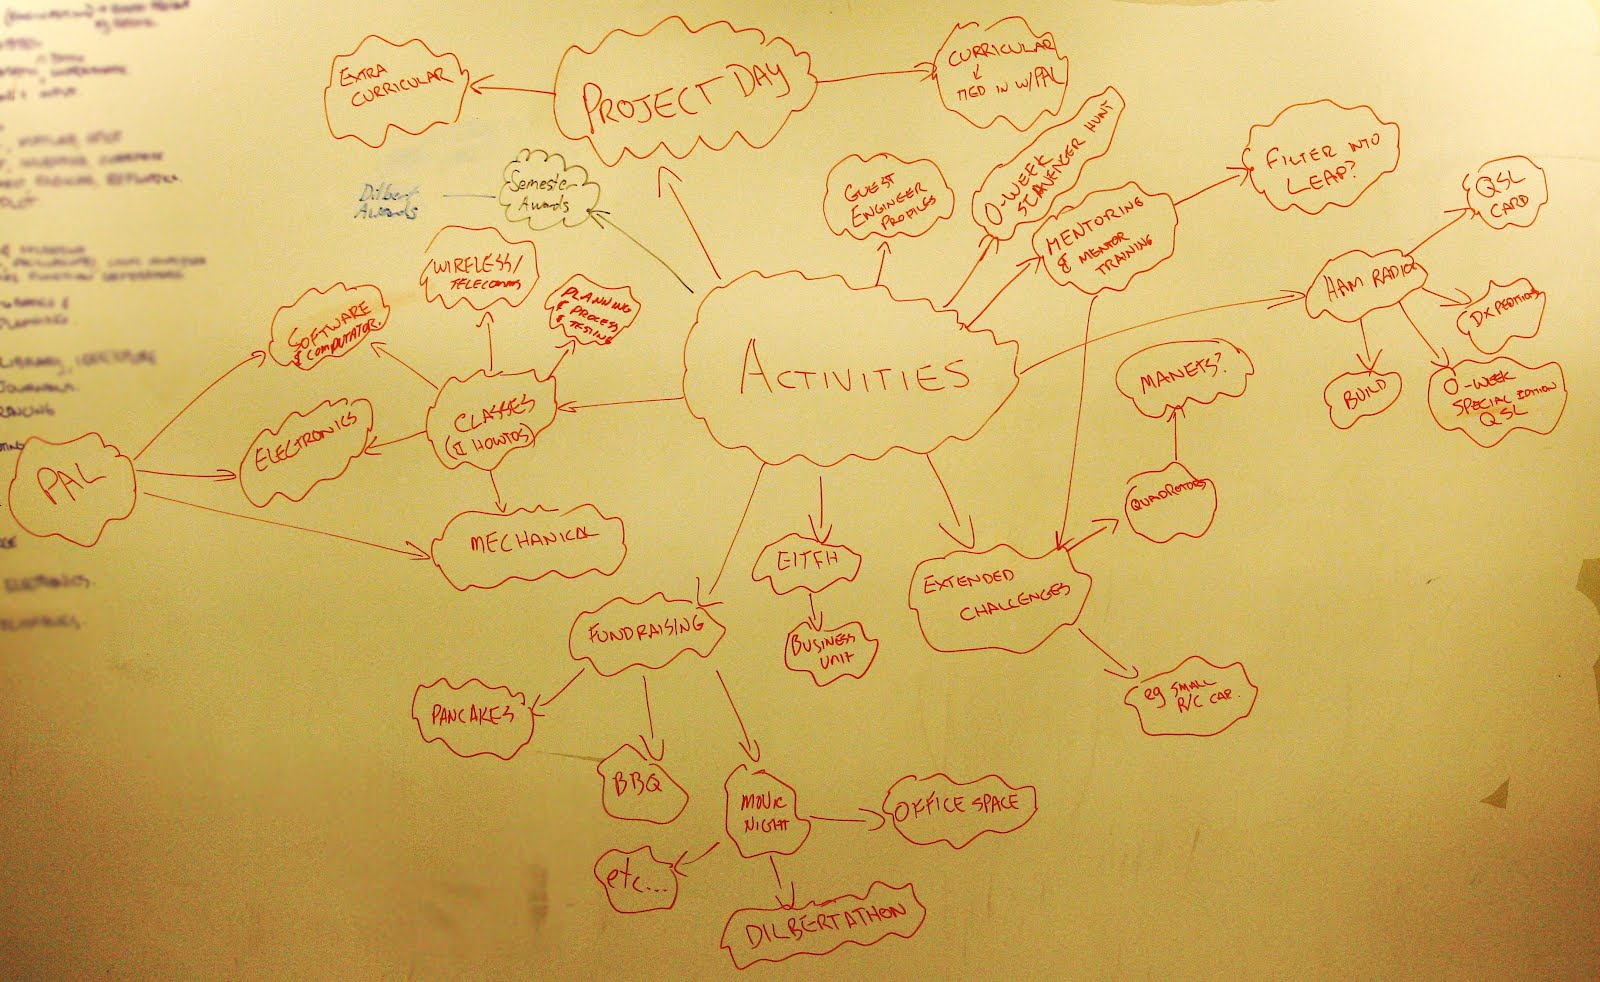
\includegraphics[angle=90, scale=0.18]{img/activities.jpg}
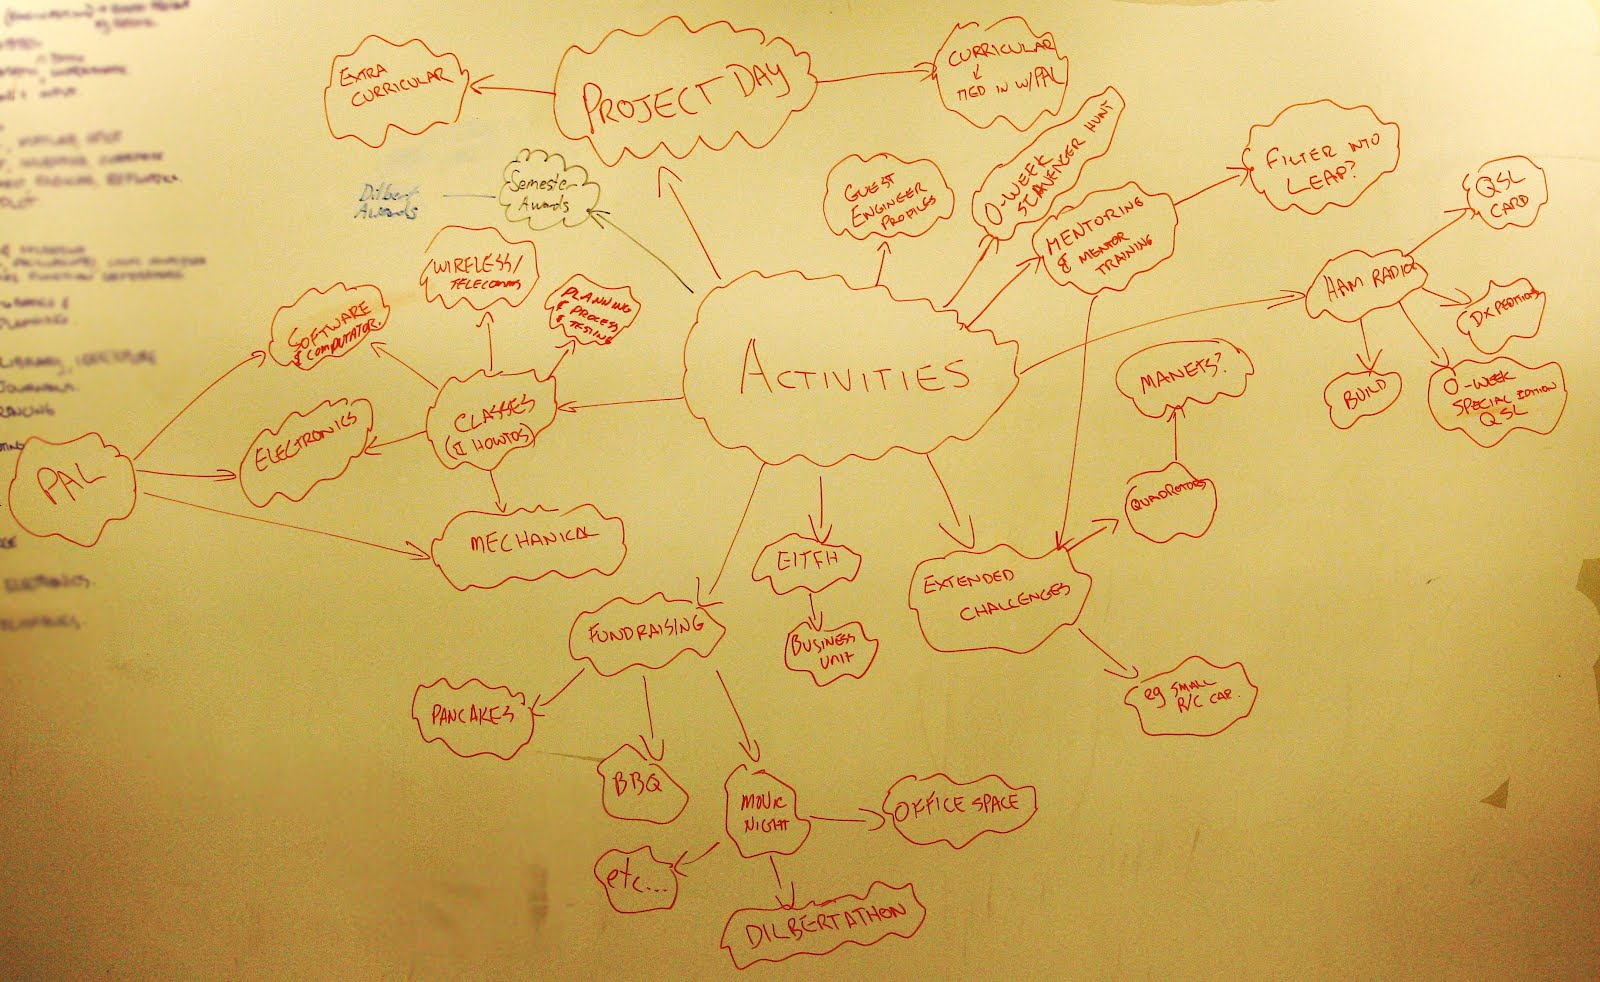
\includegraphics[angle=90, height=\textheight]{img/activities.jpg}
\subsection{Outcome}
While the possible activities is large and varied, we have identified the
following core areas:
\begin{itemize}
  \item Guest Lecturers (possibly professional engineer profiles)
  \item Classes (seminars and workshops)
  \item Project Days
  \item PAL
  \item Fundraisers
  \item Mentoring
  \item Amateur Radio
  \item Social Get togethers (Weekly)
  \item Start of year Engineering Induction with Dept of Engineering
  \item End of Semester Event (with awards)
  \item TEDx Macquarie
\end{itemize}

\subsubsection{Classes}
Classes are a large area of involvement where we would run lectures, seminars
and workshops on areas of interest, some of these are as follows:
\begin{itemize}
  \item Presentation - how to present yourself (eg resume, give talks etc)
  \item \LaTeX and BiBTeX
  \item Maths workshops geared towards engineering. (Need Mike's input)
  \item Software Tools
  \begin{itemize}
    \item AWR
    \item MATLAB
    \item SPICE
    \item OPNET
    \item Inventor
    \item Enterprise Architect
    \item EndNote
    \item Refworks
    \item GNUPLOT
  \end{itemize}
  \item UML
  \item Lab Equipment
  \begin{itemize}
    \item Use of equipment
    \item Soldering
    \item Multimeter
    \item Oscilloscopes
    \item Logic Analyser
    \item Power Supplied
    \item Function Generator
  \end{itemize}
  \item Engineering Logbooks, processes and planning (howtos)
  \item How to use resources (eg library, IEEEXplore, Journals)
  \item How to do referencing properly
  \item Embedded Computing
  \begin{itemize}
    \item Introduction (eg Arduino)
    \item Feedback Controls
  \end{itemize}
  \item EWB Challenge
  \item Funway Into Electronics
  \item Exam Preparation Techniques
\end{itemize}

\subsubsection{Social}
Social activities are also widely varied. Some options open to us:
\begin{itemize}
  \item Weekly meeting at the bar or coffee shop.
  \item Pancake / BBQ
  \item Movie Night
  \item Amateur Radio Days (in association with MQARC)
\end{itemize}

\subsubsection{PAL}
PAL (Peer Assisted Learning) is an initiative that Mike Heimlich has tried to
promote where by students assist each other in learning about engineering. It
has predominantly focused on maths, however there is no reason it cannot broaden
itself to general engineering principles such as use of lab equipment,
whiteboards, and desk space.

It would provide a place for learning through open exploration of ideas with
peers.
\include{chaps/07_academic}
\section{Finances}
\label{sec:Finances}
\subsection{Outcome}
Several ideas were presented throughout the meeting at various stages, however
the finances were never specifically addressed. The ideas which cropped up that
could be potential revenue streams:
\begin{itemize}
  \item Pancakes
  \item BBQ
  \item Movie Nights with gold coin donation
  \item Class tutorials, workshops and other activities which bear a small
  charge for non-members.
\end{itemize}

\subsection{Action Items}
\begin{itemize}
  \item Determine income and revenue strategies. Past experience tells us we
  cannot rely on MUSRA alone.
\end{itemize}
\section{Marketing}
\label{sec:Marketing}
\subsection{Outcome}
\begin{itemize}
  \item Weekly meeting at bar or coffee shop (social activity)
  \item At events
  \begin{itemize}
    \item Stalls at big events like O-Week
    \item Partnerships with other groups
  \end{itemize}
  \item Advertise in the IEEE SB Newsletter
  \item Electronic Billboards
  \item ``Robots have feelings too'' or a Wall-e at Wally's Walk to raise
  awareness and get signups.
  \item Pancake stand (\& engineering coffee display)
  \item Astronomy \& physics societies co-hosted stuffs (TBD)
  \item ``Captain Plan It?''
  \item Engineering Induction
  \item Branding, usage and templates.
\end{itemize}

\subsection{Action Items}
\begin{itemize}
  \item Choose a marketing person.
\end{itemize}
\section{Group Partnerships}
\label{sec:GroupPartnerships}
\subsection{Outcome}
Largely documented throughout other sections of this document. Summary is that
there are potential partnerships with several societies on campus:
\begin{itemize}
  \item IEEE Student Branch (not affiliated with MUSRA)
  \item Astronomy / Physics Society
  \item FIRST Alumni
  \item The following groups are not student societies, but industry
  partnerships exist with various departments and the university itself:
  \begin{itemize}
    \item APESMA
    \item Engineers Australia
    \item Engineers Without Borders
  \end{itemize}
  \item The following groups are not student societies, but various departments
  that could potentially support the society with logistical help.
  \begin{itemize}
    \item Dept of Engineering
    \item Dept of Computing
    \item Dept of Physics
    \item Dept of Astronomy
    \item Dept of Chemistry
  \end{itemize}
\end{itemize}

\subsection{Action Items}
\begin{itemize}
  \item Each partnership is a potential opportunity. Need to identify what that
  opportunity actually yields and what goals could be achieved
  \item Need to identify contacts within each partnership.
  \item Need to identify potential weaknesses
  \item Overall SWOT analysis.
\end{itemize}
\section{IT \& Communications Strategy}
\label{sec:ITComms}
\subsection{Resource Lists}
The only real area of IT \& Communications discussed was that of a list of
resources. It currently includes
\begin{itemize}
  \item Lab Equipment
  \begin{itemize}
    \item Host copies of the manuals (should copyright permit)
    \item KCMQ Activity worksheets
    \item KCMQ Quickstart Guides
    \item KCMQ Howto manuals
   \end{itemize}
  \item Setup Guides for software.
  \item Links to past papers
  \item Engineering Survival Guide
  \begin{itemize}
    \item Email addresses
    \item Websites
    \item Student Support (eg counselling)
    \item Numeracy Centre
  \end{itemize}
  \item Support videos (eg Kahn Academy)
  \item List of Engineering Research Groups
  \item Lecture Notes (from both staff and students)
\end{itemize}

\subsection{Action Items}
This was not looked into as it requires significant amount of time to think
about, as well as other details to be finalised such as resources. 
\begin{itemize}
  \item Website / social media
  \item Newsletter
  \item Membership Register
  \item Mailing list / forum
  \item Resource List
\end{itemize}
\section{Membership}
\label{sec:Membership}
\subsection{Outcome}
\subsubsection{List of Possible Members (Victims)}
Professors, Lecturers and other non-student staff members:
\begin{itemize}
  \item Sam Reisenfeld
  \item Graham Town
  \item Mike Heimlich
  \item Luan Heimlich
  \item Gangfa Feng
  \item Yinan Kong
  \item David (ELEC260)
  \item New Prof for Mechatronics Engineering
  \item Stephen Hanley
  \item Dom Verity
  \item Karu Esselle
  \item Dilshara Hill
  \item Carolyn Kennet
  \item Arun Neelakandan
  \item Darius Taslim
  \item Matt Cabanag
\end{itemize}
Postgrads:
\begin{itemize}
  \item Sayed Ali
  \item Eahteshamul Hoque
  \item Susan Bruck
  \item Ayobami Igi
  \item Forrest Zhu
  \item Barry McDonald
  \item Carl Svensson
  \item Beeshanga Abewardana Jayawickrama
  \item Audrey Markowskei
  \item Mitch Buckley
\end{itemize}
Undergrads:
\begin{itemize}
  \item Joseph Campbell
  \item Gitanjali Pradhananga
  \item Pierce Rixon
  \item Michael Griffin
  \item Zarin Saif
  \item Esther N
  \item Adam Carmichael
  \item Nathan Seal
  \item Nathaniel Hunt
  \item Tim Boye
  \item Mitch Gulliver
  \item Caroline MacDonald
  \item Gareth Richardson
  \item Joshua Larietti
  \item Tristan Allanson
  \item Rajika Kuruwita
  \item Michael Davies
  \item Adrian Kane
  \item Mat Fialkowski
  \item Chris Bagnall
  \item Chris Walker
  \item Sarah Heimlich
  \item Ben Mac
  \item Albert Chahine
\end{itemize}

\subsection{Action Items}
\begin{itemize}
  \item Approach above personnel with invitations to join and form a group, and
  to request their help.
  \item Staff members need to be asked with personalized invitations, perhaps
  over a cup of coffee.
  \item Some students are earmarked for committee positions, these people need
  to be invited specifically once roles are determined  kjl
  \item Do we charge a fee?
\end{itemize}


\end{document}